\chapter{समष्टि आनुवंशिकी और प्राकृतिक वरण}\label{ch:b2:population-genetics}

1848 में मैनचेस्टर के पास कोई काला मिर्चदार पतंगा पकड़ा गया; 1895 तक
उस शहर में बीस में से उन्नीस पतंगे काले थे, और 1970 तक, ज्यों-ज्यों वह कालिख
गई, वह पीला रूप लौट आया। वे पतंगे नहीं बदले: लाखों की किसी समष्टि में
दो युग्मविकल्पियों के अनुपात बदले, वह भी चिड़ियों की आँखों के नीचे,
कुछ दर्जन पीढ़ियों में। डार्विन ने देख लिया था कि वरण को
जातियाँ बदलनी ही होंगी पर उसे गिनने का उनके पास कोई रास्ता न था;
वह गिनना \omterm{def:b2:population-genetics:frequencies}{समष्टि आनुवंशिकी} है, और वही इस अध्याय का अंकगणित है।
वह पूछता है कि जब उन पर कुछ भी काम न करे तब युग्मविकल्पी-बारंबारताएँ कैसा
बर्ताव करती हैं, और फिर वरण, \omterm{def:b2:genome-diversification:mutation}{उत्परिवर्तन}, प्रवास, संयोग तथा
अंतःप्रजनन उन्हें कितनी तेज़ी से हिलाते हैं --- और वह उन लक्षणों पर अंत होता है जो
एक जीन नहीं बल्कि कई हैं, और वही अधिकांश है जो वरण असल में
देखता है।

\section{विश्राम में जीन-कोष}

\begin{definition}[समष्टि, जीन-कोष, बारंबारताएँ]\label{def:b2:population-genetics:frequencies}
\index{समष्टि आनुवंशिकी}\index{जीन-कोष}\index{युग्मविकल्पी बारंबारता}
\emph{समष्टि} एक ही जाति के ऐसे व्यष्टियों का समूह है जो आपस में
प्रजनन करते हैं; और उसका \emph{जीन-कोष} उनके सारे युग्मविकल्पियों का समुच्चय है।
दो युग्मविकल्पियों $A$ तथा $a$ वाले किसी स्थल के लिए, $N$ व्यष्टियों की
किसी \omterm{def:b2:meiosis-heredity:meiosis}{द्विगुणित} समष्टि में, \emph{\omterm{def:b2:meiosis-heredity:vocabulary}{युग्मविकल्पी} बारंबारताएँ} $p = (2N_{AA} +
N_{Aa})/2N$ तथा $q = 1 - p$ हैं, और \emph{\omterm{def:b2:meiosis-heredity:vocabulary}{जीन-प्ररूप} बारंबारताएँ}
$AA$, $Aa$ तथा $aa$ के अंश हैं। सबसे सँकरे अर्थ में
विकास पीढ़ियों के बीच युग्मविकल्पी-बारंबारताओं का परिवर्तन है; और इस
अध्याय का प्रश्न यह है कि उन्हें क्या और कितना बदलता है।
\end{definition}

\begin{theorem}[हार्डी--वाइनबर्ग]\label{thm:b2:population-genetics:hw}
\index{हार्डी--वाइनबर्ग नियम}
यादृच्छिक रूप से प्रजनन करती किसी बड़ी समष्टि में, बिना वरण, \omterm{def:b2:genome-diversification:mutation}{उत्परिवर्तन}
या प्रवास के, युग्मविकल्पी-बारंबारताएँ एक पीढ़ी से
अगली तक नहीं बदलतीं, और यादृच्छिक प्रजनन की एक ही पीढ़ी के बाद
\omterm{def:b2:meiosis-heredity:vocabulary}{जीन-प्ररूप} बारंबारताएँ ये हैं:
\[
AA : p^{2}, \qquad Aa : 2pq, \qquad aa : q^{2},
\]
और ऐसी ही बनी रहती हैं। प्रभाविता किसी \omterm{def:b2:meiosis-heredity:vocabulary}{प्रभावी} \omterm{def:b2:meiosis-heredity:vocabulary}{युग्मविकल्पी} को फैला नहीं देती, और
कोई दुर्लभ \omterm{def:b2:meiosis-heredity:vocabulary}{अप्रभावी} \omterm{def:b2:meiosis-heredity:vocabulary}{युग्मविकल्पी} खोता नहीं: वह विषमयुग्मजों में छिपता है,
जो समयुग्मजों से $2p/q$ गुना अधिक हैं --- $q = 0.01$ के लिए,
दो सौ गुना। वह नियम \omterm{def:b2:population-genetics:frequencies}{समष्टि आनुवंशिकी} की शून्य
परिकल्पना है: किसी असली समष्टि में उससे कोई विचलन, या पीढ़ियों के बीच
$p$ का कोई परिवर्तन, नीचे दिए बलों में से किसी एक का
हस्ताक्षर है।
\end{theorem}
\begin{proof}
यादृच्छिक प्रजनन युग्मकों का यादृच्छिक मिलन है: कोई युग्मक $A$
प्रायिकता $p$ से और $a$ प्रायिकता $q$ से ढोता है, अपने
साथी से स्वतंत्र रूप से, इसलिए वह युग्मनज $AA$ है प्रायिकता $p^{2}$ से, $Aa$
$2pq$ से, और $aa$ $q^{2}$ से। अगली पीढ़ी में \omterm{def:b2:population-genetics:frequencies}{युग्मविकल्पी बारंबारता}
$p' = p^{2} + \tfrac12(2pq) = p(p + q) = p$ है: यानी अपरिवर्तित।
चूँकि वे \omterm{def:b2:meiosis-heredity:vocabulary}{जीन-प्ररूप} बारंबारताएँ केवल $p$ पर निर्भर हैं, इसलिए वे पहली के बाद
हर पीढ़ी में वही हैं।
\end{proof}

\begin{example}[कोई बारंबारता पढ़ना]\label{ex:b2:population-genetics:cf}
पुटीय तंतुमयता, जो \omterm{def:b2:meiosis-heredity:vocabulary}{अप्रभावी} है, 2500 में से एक यूरोपीय बच्चे को होती है:
$q^{2} = 1/2500$, $q = 0.02$, और वाहक-बारंबारता $2pq
\approx 0.04$ --- यानी 25 में से एक व्यक्ति ऐसा \omterm{def:b2:meiosis-heredity:vocabulary}{युग्मविकल्पी} ढोता है जो अपने
समयुग्मजों को मार डालता है, और उस \omterm{def:b2:meiosis-heredity:vocabulary}{युग्मविकल्पी} की प्रतियों का \qty{98}{\%}
स्वस्थ वाहकों में बैठा है जहाँ वरण उन्हें देख नहीं सकता। इसीलिए कोई
घातक \omterm{def:b2:meiosis-heredity:vocabulary}{अप्रभावी} इतनी धीरे हटाया जाता है, और इसीलिए प्रभावितों की नसबंदी करके
\omterm{def:b2:meiosis-heredity:vocabulary}{अप्रभावी} रोग मिटाने की सुजननकी योजनाएँ कभी
चल ही नहीं सकती थीं: अगले खंड का अंकगणित दिखाता है कि कितनी
धीरे।
\end{example}

\section{वरण}

\begin{definition}[अनुकूलता]\label{def:b2:population-genetics:fitness}
\index{अनुकूलता}\index{वरण गुणांक}
किसी \omterm{def:b2:meiosis-heredity:vocabulary}{जीन-प्ररूप} की \emph{अनुकूलता} $w$ अगली पीढ़ी में संतति का उसका
सापेक्ष अंशदान है --- यानी प्रजनन तक उत्तरजीविता
गुणा जननक्षमता, और वह भी ऐसे पैमाने पर कि सर्वोत्तम \omterm{def:b2:meiosis-heredity:vocabulary}{जीन-प्ररूप} की $w = 1$ हो।
किसी \omterm{def:b2:meiosis-heredity:vocabulary}{जीन-प्ररूप} का \emph{वरण गुणांक} $s$ उसकी कमी है,
$w = 1 - s$। अनुकूलता किसी पर्यावरण में किसी \omterm{def:b2:meiosis-heredity:vocabulary}{जीन-प्ररूप} का गुण है,
न कि स्वयं किसी \omterm{def:b2:meiosis-heredity:vocabulary}{युग्मविकल्पी} का: काले पतंगे के \omterm{def:b2:meiosis-heredity:vocabulary}{युग्मविकल्पी} की, पीले के सापेक्ष,
कालिख भरी \omterm{def:b2:plant-meristems:wood}{छाल} पर $w > 1$ थी और शैवाकों पर $w < 1$।
\end{definition}

\begin{theorem}[वरण युग्मविकल्पी बारंबारता बदलता है]\label{thm:b2:population-genetics:selection}
\index{प्राकृतिक वरण!समीकरण}
\omterm{def:b2:meiosis-heredity:vocabulary}{जीन-प्ररूप} \omterm{def:b2:population-genetics:fitness}{अनुकूलताओं} $w_{AA}$, $w_{Aa}$, $w_{aa}$ के साथ माध्य
\omterm{def:b2:population-genetics:fitness}{अनुकूलता} $\bar w = p^{2}w_{AA} + 2pq\,w_{Aa} + q^{2}w_{aa}$ है और अगली पीढ़ी में
\omterm{def:b2:population-genetics:frequencies}{युग्मविकल्पी बारंबारता} है
\[
p' = \frac{p^{2}w_{AA} + pq\,w_{Aa}}{\bar w}, \qquad
\Delta p = p' - p = \frac{pq\,\bigl[p(w_{AA} - w_{Aa}) + q(w_{Aa} - w_{aa})\bigr]}{\bar w}.
\]
दो परिणाम। पहला, $\Delta p$ $pq$ के समानुपाती है: वरण
मध्यवर्ती बारंबारताओं पर सबसे तेज़ है और तब सबसे धीमा जब कोई \omterm{def:b2:meiosis-heredity:vocabulary}{युग्मविकल्पी}
दुर्लभ हो या लगभग नियत --- वहाँ उस पर काम करने को थोड़ी ही विविधता है।
दूसरा, किसी \omterm{def:b2:meiosis-heredity:vocabulary}{अप्रभावी} \omterm{def:b2:meiosis-heredity:vocabulary}{युग्मविकल्पी} के विरुद्ध ($w_{AA} = w_{Aa} = 1$, $w_{aa} =
1 - s$) वह परिवर्तन $\Delta q = -s\,pq^{2}/\bar w$ है, यानी
$q^{2}$ के समानुपाती: कोई दुर्लभ \omterm{def:b2:meiosis-heredity:vocabulary}{अप्रभावी} वरण को लगभग अदृश्य है, और
उसकी बारंबारता $0.01$ से आधी करने में लगभग सौ पीढ़ियाँ लगती हैं
तब भी जब उसके समयुग्मज घातक हों। कोई अनुकूल \omterm{def:b2:meiosis-heredity:vocabulary}{प्रभावी} \omterm{def:b2:meiosis-heredity:vocabulary}{युग्मविकल्पी}
पहले तेज़ फैलता है और फिर अंत में रुक जाता है, उसी
कारण से।
\end{theorem}
\begin{proof}
उस संतति में से अंश $p^{2}w_{AA}/\bar w$ $AA$ है और
$2pq\,w_{Aa}/\bar w$ $Aa$ (हर \omterm{def:b2:meiosis-heredity:vocabulary}{जीन-प्ररूप} की बारंबारता उसकी
\omterm{def:b2:population-genetics:fitness}{अनुकूलता} से भारित तथा फिर से सामान्यित); और उनमें $A$ \omterm{def:b2:meiosis-heredity:vocabulary}{युग्मविकल्पी} पहले के सारे
और दूसरे के आधे हैं, जो $p'$ देते हैं। $p =
p\bar w/\bar w$ घटाने और $\bar w$ फैलाने से $\Delta p$ मिलता है। किसी घातक
\omterm{def:b2:meiosis-heredity:vocabulary}{अप्रभावी} के लिए ($s = 1$): $q' = q^{2}\cdot 0 + pq$ बँटा $\bar w = 1 -
q^{2}$, इसलिए $q' = q/(1 + q)$, जिससे $1/q' = 1/q + 1$ और $t$
पीढ़ियों बाद $1/q_t = 1/q_0 + t$: यानी $q_0 = 0.01$ से $0.005$ तक
$t = 100$ लगता है।
\end{proof}

\begin{omfigure}
\begin{tikzpicture}
\begin{axis}[
  width=0.8\linewidth, height=6cm,
  axis x line=bottom, axis y line=left,
  xmin=0, xmax=150, ymin=0, ymax=1.05,
  xlabel={पीढ़ियाँ}, ylabel={अनुकूल युग्मविकल्पी की बारंबारता},
  xlabel style={font=\small, at={(axis description cs:0.5,-0.11)}, anchor=north},
  ylabel style={font=\small},
  tick label style={font=\small}, xtick={0,50,100,150}, ytick={0,0.5,1},
  legend style={font=\scriptsize, at={(0.97,0.35)}, anchor=east, draw=none},
  clip=false,
]
\addplot[very thick, omDef] table[x=t, y=dom] {
t dom
0 0.01
10 0.02
20 0.04
30 0.075
40 0.14
50 0.24
60 0.38
70 0.53
80 0.66
90 0.76
100 0.83
110 0.88
120 0.91
130 0.93
140 0.945
150 0.955
};
\addlegendentry{अनुकूल युग्मविकल्पी प्रभावी, $s = 0.1$}
\addplot[very thick, omThm] table[x=t, y=rec] {
t rec
0 0.01
10 0.0101
20 0.0102
30 0.0104
40 0.0106
50 0.0108
60 0.011
70 0.0113
80 0.0116
90 0.012
100 0.0124
110 0.0128
120 0.0133
130 0.0138
140 0.0144
150 0.015
};
\addlegendentry{अनुकूल युग्मविकल्पी अप्रभावी, $s = 0.1$}
\end{axis}
\end{tikzpicture}

{\small \qty{10}{\%} के किसी लाभ के साथ वरण काम पर। कोई अनुकूल
\omterm{def:b2:meiosis-heredity:vocabulary}{प्रभावी} \omterm{def:b2:meiosis-heredity:vocabulary}{युग्मविकल्पी} सत्तर पीढ़ियों में \qty{1}{\%} से चढ़कर बहुमत हो जाता है
और फिर धीमा पड़ता है, जबकि उसका दुर्लभ \omterm{def:b2:meiosis-heredity:vocabulary}{अप्रभावी} प्रतिद्वंद्वी
विषमयुग्मजों में छिपा रहता है; और \qty{1}{\%} पर कोई अनुकूल \omterm{def:b2:meiosis-heredity:vocabulary}{अप्रभावी} \omterm{def:b2:meiosis-heredity:vocabulary}{युग्मविकल्पी} उसी समय में मुश्किल से
हिलता है, क्योंकि वह लगभग कभी उघड़ता ही नहीं।}
\end{omfigure}

\begin{proposition}[वरण के प्रकार]\label{prop:b2:population-genetics:kinds}
\index{दिशात्मक वरण}\index{स्थायीकारी वरण}\index{संतुलनकारी वरण}\index{विषमयुग्मज लाभ}
\emph{दिशात्मक} वरण किसी एक छोर को अनुकूल पाता है और किसी
\omterm{def:b2:meiosis-heredity:vocabulary}{युग्मविकल्पी} को नियतन की ओर चलाता है (कालिख भरे वन में वह काला पतंगा; प्रतिजैविक
प्रतिरोध; किसी सूखे में किसी फ़िंच की चोंच का आकार)।
\emph{स्थायीकारी} वरण बीच को अनुकूल पाता है और उन
छोरों को हटाता है (मानव जन्म-भार: जो शिशु मरते हैं वे सबसे छोटे
और सबसे बड़े हैं); वह किसी समष्टि को जहाँ है वहीं रखता है और सबसे आम प्रकार है।
\emph{विदारक} वरण बीच के विरुद्ध दोनों छोरों को अनुकूल पाता है,
और किसी समष्टि को बाँट सकता है
(\cref{ch:b2:speciation})। \emph{संतुलनकारी} वरण दो
युग्मविकल्पियों को उस समष्टि में अनिश्चित काल तक रखता है: \emph{\omterm{prop:b2:population-genetics:kinds}{विषमयुग्मज
लाभ}} से, जब $Aa$ दोनों समयुग्मजों से अधिक अनुकूल हो --- और
$w_{AA} = 1 - s$, $w_{aa} = 1 - t$, $w_{Aa} = 1$ के साथ वह बारंबारता
$\hat p = t/(s + t)$ पर बैठ जाती है --- या \emph{बारंबारता-निर्भर}
वरण से, जब कोई \omterm{def:b2:meiosis-heredity:vocabulary}{जीन-प्ररूप} जितना दुर्लभ हो उतना अधिक अनुकूल हो (
\cref{ch:b2:angiosperm-reproduction} के दुर्लभ $S$ \omterm{def:b2:meiosis-heredity:vocabulary}{युग्मविकल्पी}, ऐसा शिकार
जिसे कोई परभक्षी सीखा न हो, किसी शल्क-भक्षी मछली के मुँह के दोनों पार्श्व)।
\end{proposition}
\begin{proof}[प्रमाण-सामग्री]
हँसिया-कोशिका हीमोग्लोबिन अधिकांश समयुग्मजों को उनके प्रजनन से पहले मार
देता है, फिर भी वह \omterm{def:b2:meiosis-heredity:vocabulary}{युग्मविकल्पी} मलेरिया वाले अफ़्रीका भर
\qty{10}{\%} से \qty{20}{\%} पर है। ऐलिसन (1954) ने दिखाया कि \omterm{def:b2:meiosis-heredity:vocabulary}{विषमयुग्मजी} बच्चों को
दोनों समयुग्मजों में से किसी से भी कहीं कम तथा हलके मलेरिया-संक्रमण होते
थे, और उस \omterm{def:b2:meiosis-heredity:vocabulary}{युग्मविकल्पी} की बारंबारता फ़ैल्सीपेरम मलेरिया के ऐतिहासिक
वितरण पर बैठती है; और अफ़्रीकी वंश की जिन समष्टियों में
मलेरिया नहीं है वहाँ वह बारंबारता तब से गिरती रही है। किसी मलेरिया वाले क्षेत्र में
हँसिया समयुग्मज के लिए $t \approx 0.8$ और सामान्य समयुग्मज के लिए $s \approx 0.1$ के साथ,
$\hat q = s/(s + t) \approx 0.11$ --- यानी जो देखा जाता है।
\end{proof}

\section{उत्परिवर्तन, प्रवास, और वह संतुलन}

\begin{theorem}[उत्परिवर्तन--वरण संतुलन]\label{thm:b2:population-genetics:balance}
\index{उत्परिवर्तन--वरण संतुलन}\index{आनुवंशिक भार}
कोई हानिकर \omterm{def:b2:meiosis-heredity:vocabulary}{युग्मविकल्पी} प्रति युग्मक प्रति पीढ़ी $\mu$ दर से \omterm{def:b2:genome-diversification:mutation}{उत्परिवर्तन} से
पोसा जाता है और वरण से हटाया जाता है। साम्य पर वे दोनों
संतुलित होते हैं: $s$ \omterm{def:b2:meiosis-heredity:vocabulary}{समयुग्मजी} हानि वाले किसी \omterm{def:b2:meiosis-heredity:vocabulary}{अप्रभावी} \omterm{def:b2:meiosis-heredity:vocabulary}{युग्मविकल्पी} के लिए,
\[
\hat q = \sqrt{\mu/s}\,;
\]
और $hs$ \omterm{def:b2:meiosis-heredity:vocabulary}{विषमयुग्मजी} हानि वाले किसी \omterm{def:b2:meiosis-heredity:vocabulary}{प्रभावी} (या आंशिक रूप से \omterm{def:b2:meiosis-heredity:vocabulary}{प्रभावी}) \omterm{def:b2:meiosis-heredity:vocabulary}{युग्मविकल्पी}
के लिए, $\hat q = \mu/hs$। इस तरह किसी
\omterm{def:b2:meiosis-heredity:vocabulary}{अप्रभावी} की साम्य बारंबारता किसी घातक के लिए भी बड़ी है: $\mu = 10^{-5}$ तथा
$s = 1$ के साथ, $\hat q = 3\times 10^{-3}$, और उस समष्टि का \qty{0.6}{\%}
उसे ढोता है। हर समष्टि हज़ारों स्थलों पर ऐसा कोई \emph{\omterm{thm:b2:population-genetics:balance}{आनुवंशिक भार}}
ढोती है, जिसका अधिकांश \omterm{def:b2:meiosis-heredity:vocabulary}{अप्रभावी} तथा छिपा है, और
\cref{ch:b2:asexual-reproduction} के रैचेट-तर्क का वह साम्य
--- यानी व्यष्टियों का कोई अंश $e^{-U/s}$ जो हानिकर
\omterm{def:b2:genome-diversification:mutation}{उत्परिवर्तनों} से मुक्त है --- वही संतुलन है, जीनोम भर जोड़ा हुआ।
\end{theorem}
\begin{proof}
हर पीढ़ी \omterm{def:b2:genome-diversification:mutation}{उत्परिवर्तन} $\mu p \approx \mu$ को $q$ में जोड़ता है और
वरण $s\,pq^{2}/\bar w \approx sq^{2}$ हटाता है (छोटी $q$ के लिए);
$\mu = s\hat q^{2}$ रखने से वह \omterm{def:b2:meiosis-heredity:vocabulary}{अप्रभावी} परिणाम मिलता है। किसी
\omterm{def:b2:meiosis-heredity:vocabulary}{प्रभावी} \omterm{def:b2:meiosis-heredity:vocabulary}{युग्मविकल्पी} के लिए वरण प्रति पीढ़ी $hs\,q$ हटाता है (हर प्रति
किसी विषमयुग्मज में उघड़ी है), और $\mu = hs\hat q$।
\end{proof}

\begin{proposition}[प्रवास और एक-प्रवासी नियम]\label{prop:b2:population-genetics:migration}
\index{जीन-प्रवाह}\index{प्रवास (आनुवंशिक)}
यदि किसी समष्टि का कोई अंश $m$ हर पीढ़ी ऐसी किसी समष्टि से आए प्रवासी हों
जिसकी \omterm{def:b2:population-genetics:frequencies}{युग्मविकल्पी बारंबारता} $p_{m}$ हो, तो वह बारंबारता $p_{m}$ की ओर
$\Delta p = m(p_{m} - p)$ से चलती है: और दोनों समष्टियों के बीच का
अंतर $(1 - m)^{t}$ की तरह क्षीण होता है।
\emph{\omterm{prop:b2:population-genetics:migration}{जीन-प्रवाह}} समांगी करता है; वह स्थानीय \omterm{def:b2:plant-plasticity:plasticity}{अनुकूलन} उलट देता है जब तक वरण
$m$ से मज़बूत न हो, और वही वह बल है जो किसी जाति को एक ही
जाति बनाए रखता है। उलटे, कोई प्रवासी न बदलती समष्टियाँ
अपवाह से तथा अपने अलग-अलग \omterm{def:b2:genome-diversification:mutation}{उत्परिवर्तनों} से विचलित होती हैं, और प्रति पीढ़ी कोई एक
प्रवासी --- समष्टि का आकार जो भी हो --- उन्हें भिन्न युग्मविकल्पियों के लिए
नियतन तक अपवाहित होने से रोकने भर को काफ़ी है।
\end{proposition}

\section{संयोग: आनुवंशिक अपवाह}

\begin{theorem}[आनुवंशिक अपवाह]\label{thm:b2:population-genetics:drift}
\index{आनुवंशिक अपवाह}\index{प्रभावी समष्टि आकार}\index{नियतन}
$N$ \omterm{def:b2:meiosis-heredity:meiosis}{द्विगुणित} व्यष्टियों की किसी समष्टि में हर पीढ़ी की
\omterm{def:b2:population-genetics:frequencies}{युग्मविकल्पी बारंबारता} पिछली से $2N$ युग्मकों का कोई यादृच्छिक प्रतिदर्श है,
इसलिए $p$ प्रति पीढ़ी $p(1 - p)/2N$ के प्रसरण के साथ यादृच्छिक भटकता है।
\emph{विषमयुग्मजता} $H = 2pq$ हर पीढ़ी औसतन
$(1 - 1/2N)$ गुणक से क्षीण होती है,
\[
H_t = H_0\left(1 - \frac{1}{2N}\right)^{t} \approx H_0\,e^{-t/2N},
\]
और हर \omterm{def:b2:meiosis-heredity:vocabulary}{युग्मविकल्पी} अंततः खो जाता है या \emph{नियत} हो जाता है, और वह भी
अपनी वर्तमान बारंबारता के बराबर प्रायिकता से: कोई नया उदासीन \omterm{def:b2:genome-diversification:mutation}{उत्परिवर्तन},
जो $1/2N$ बारंबारता पर है, प्रायिकता $1/2N$ से नियत होता है और, यदि होता है, तो
उसमें लगभग $4N$ पीढ़ियाँ लेता है। अपवाह लाखों की किसी
समष्टि में नगण्य है और दर्जनों की किसी में \omterm{def:b2:meiosis-heredity:vocabulary}{प्रभावी}: कोई
\emph{अड़चन} या कोई \emph{संस्थापक} घटना --- किसी द्वीप पर कुछ उपनिवेशी, या
शिकार से सौ भर तक घटाई गई कोई जाति --- पीढ़ी भर में संयोग से \omterm{def:b2:meiosis-heredity:vocabulary}{युग्मविकल्पी}
खो देती है और ऐसी समष्टि छोड़ जाती है जो एकरूप,
दरिद्र तथा समयुग्मजों से भरी है। जो $N$ मायने रखता है वह
\emph{\omterm{def:b2:meiosis-heredity:vocabulary}{प्रभावी}} आकार है, यानी असल में प्रजनन करते व्यष्टियों की संख्या,
जो आम तौर पर जनगणना से कहीं छोटी है।
\end{theorem}
\begin{proof}
अगली पीढ़ी की $2N$ जीन-प्रतियाँ ऐसे कोष से प्रतिस्थापन के साथ खींची जाती
हैं जिसमें $A$ की बारंबारता $p$ है: $A$ प्रतियों की संख्या
माध्य $2Np$ तथा प्रसरण $2Np(1 - p)$ के साथ द्विपद है, इसलिए $p'$ का
माध्य $p$ और प्रसरण $p(1 - p)/2N$ है। अगली पीढ़ी में यादृच्छिक रूप से खींची
गई दो प्रतियाँ प्रायिकता $1/2N$ से उसी जनक-प्रति से आती हैं
और तब एकसमान हैं, इसलिए यह संभावना कि दो
प्रतियाँ भिन्न हों (यानी वह विषमयुग्मजता) हर पीढ़ी $1 - 1/2N$ से
गुणा हो जाती है। नियतन-प्रायिकता: किसी उदासीन \omterm{def:b2:meiosis-heredity:vocabulary}{युग्मविकल्पी} की बारंबारता कोई
मार्टिंगेल है --- उसका प्रत्याशित मान कभी नहीं बदलता --- और वह 0
या 1 पर अंत होती है, इसलिए 1 पर अंत होने की प्रायिकता उसके आरंभिक मान के बराबर है।
\end{proof}

\begin{omfigure}
\begin{tikzpicture}
\begin{axis}[
  width=0.82\linewidth, height=6cm,
  axis x line=bottom, axis y line=left,
  xmin=0, xmax=60, ymin=0, ymax=1.05,
  xlabel={पीढ़ियाँ}, ylabel={युग्मविकल्पी बारंबारता $p$},
  xlabel style={font=\small, at={(axis description cs:0.5,-0.11)}, anchor=north},
  ylabel style={font=\small},
  tick label style={font=\small}, xtick={0,20,40,60}, ytick={0,0.5,1},
  legend style={font=\scriptsize, at={(0.5,-0.25)}, anchor=north, draw=none, legend columns=2},
  clip=false,
]
\addplot[thick, omThm] coordinates {(0,0.5) (2,0.55) (4,0.62) (6,0.58) (8,0.7) (10,0.8) (12,0.75) (14,0.85) (16,0.92) (18,0.88) (20,0.95) (22,1) (60,1)};
\addlegendentry{$N = 10$}
\addplot[thick, omThm!60] coordinates {(0,0.5) (2,0.42) (4,0.35) (6,0.4) (8,0.3) (10,0.2) (12,0.25) (14,0.15) (16,0.1) (18,0.05) (20,0.08) (22,0.02) (24,0) (60,0)};
\addplot[thick, omDef] coordinates {(0,0.5) (5,0.52) (10,0.49) (15,0.53) (20,0.56) (25,0.54) (30,0.58) (35,0.55) (40,0.57) (45,0.6) (50,0.58) (55,0.61) (60,0.6)};
\addlegendentry{$N = 1000$}
\addplot[thick, omDef!60] coordinates {(0,0.5) (5,0.48) (10,0.5) (15,0.47) (20,0.45) (25,0.46) (30,0.44) (35,0.45) (40,0.43) (45,0.44) (50,0.42) (55,0.43) (60,0.42)};
\end{axis}
\end{tikzpicture}

{\small अपवाह। दस व्यष्टियों की दो समष्टियाँ, जो
$p = 0.5$ से शुरू होती हैं, पच्चीस पीढ़ियों के भीतर उलटे \omterm{def:b2:meiosis-heredity:vocabulary}{युग्मविकल्पी} नियत करती हैं; जबकि
हज़ार की दो साठ में कुछ प्रतिशत भर भटकती हैं।}
\end{omfigure}

\begin{proposition}[अंतःप्रजनन]\label{prop:b2:population-genetics:inbreeding}
\index{अंतःप्रजनन}\index{अंतःप्रजनन गुणांक}\index{अंतःप्रजनन अवसाद}
संबंधियों के बीच प्रजनन युग्मविकल्पी-बारंबारताएँ नहीं बदलता पर
समयुग्मजों का अनुपात चढ़ा देता है: किसी व्यष्टि का
\emph{\omterm{prop:b2:population-genetics:inbreeding}{अंतःप्रजनन गुणांक}} $F$ वह प्रायिकता है कि किसी स्थल पर उसके दोनों
\omterm{def:b2:meiosis-heredity:vocabulary}{युग्मविकल्पी} वंश से एकसमान हों, और वे \omterm{def:b2:meiosis-heredity:vocabulary}{जीन-प्ररूप}
बारंबारताएँ $p^{2} + Fpq$, $2pq(1 - F)$, $q^{2} + Fpq$ हो जाती हैं।
पहले चचेरे भाई-बहनों की संतति के लिए $F = 1/16$, सहोदरों की के लिए $1/4$, और
स्व-निषेचन की के लिए $1/2$। चूँकि \omterm{thm:b2:population-genetics:balance}{आनुवंशिक भार} के \omterm{def:b2:meiosis-heredity:vocabulary}{अप्रभावी} \omterm{def:b2:meiosis-heredity:vocabulary}{युग्मविकल्पी}
उन अतिरिक्त समयुग्मजों में उघड़ते हैं, इसलिए अंतःप्रजनित संतति
\emph{\omterm{prop:b2:population-genetics:inbreeding}{अंतःप्रजनन अवसाद}} भोगती है: $q = 0.01$ पर कोई घातक \omterm{def:b2:meiosis-heredity:vocabulary}{अप्रभावी}
यादृच्छिक प्रजनन की संतति के $q^{2} = 10^{-4}$ में प्रकट होता है पर
चचेरों के बच्चों के $q^{2} + Fpq = 7\times 10^{-4}$ में, यानी सात गुना अधिक;
और हज़ारों स्थलों पर जोड़ा जाए तो चचेरों के बच्चों की शिशु-मृत्यु दूसरों से लगभग
दुगुनी है, और कोई छोटी समष्टि जो पीढ़ियों तक अंतःप्रजनन करे
जननक्षमता तथा ओज खो देती है --- यानी चीते, फ़्लोरिडा-प्यूमा
तथा यूरोप के राजवंशों की दुर्दशा।
\end{proposition}

\section{बहुत-से जीन: मात्रात्मक लक्षण}

\begin{theorem}[वंशागतिता और वरण की अनुक्रिया]\label{thm:b2:population-genetics:heritability}
\index{वंशागतिता}\index{मात्रात्मक आनुवंशिकी}\index{प्रजनक-समीकरण}
ऊँचाई, उपज या चोंच की गहराई जैसा कोई लक्षण छोटे प्रभाव वाले बहुत-से
जीनों से तथा उस पर्यावरण से बैठता है, और वह
सतत रूप से बदलता है। किसी समष्टि में उसका प्रसरण किसी
\emph{आनुवंशिक} भाग $V_G$ और किसी \emph{पर्यावरणीय} भाग $V_E$ में बँटता है, और
\emph{वंशागतिता} $h^{2} = V_A/V_P$ उस लक्षणप्ररूपी प्रसरण का वह अंश है जो
जीनों के योगात्मक प्रभावों से आता है (यानी वह भाग
जो संचरित होता है)। यदि अगली पीढ़ी के जनक ऐसे माध्य से वरे जाएँ जो उस
समष्टि के माध्य से $S$ अधिक हो (यानी वह
\emph{वरण अंतर}), तो उनकी संतति उससे इतनी अधिक होती है:
\[
R = h^{2}\,S
\]
--- यानी वह \emph{\omterm{thm:b2:population-genetics:heritability}{प्रजनक-समीकरण}}। वह एक ही पंक्ति में सारा प्राणी- तथा
पादप-प्रजनन है: $0.5$ की कोई वंशागतिता और माध्य से एक
मानक विचलन ऊपर के जनक ऐसी संतति देते हैं जो उससे आधा मानक विचलन
ऊपर है, और वह लाभ पीढ़ी-दर-पीढ़ी जमा होता है।
वंशागतिता किसी पर्यावरण में किसी समष्टि का गुण है, न कि किसी
लक्षण का: वह इस बारे में कुछ नहीं कहती कि कोई लक्षण नियत है या नहीं,
और किसी एक समष्टि में $h^{2} = 0.8$ वाले किसी लक्षण की किसी दूसरी में, जहाँ हर व्यष्टि का वही
\omterm{def:b2:meiosis-heredity:vocabulary}{जीन-प्ररूप} हो, $h^{2} = 0$ हो सकती है।
\end{theorem}
\begin{proof}
संतति का प्रत्याशित \omterm{def:b2:meiosis-heredity:vocabulary}{लक्षण-प्ररूप} मध्य-जनक के \omterm{def:b2:meiosis-heredity:vocabulary}{लक्षण-प्ररूप} पर
ढाल $h^{2}$ से समाश्रित है (यानी संबंधियों के बीच योगात्मक आनुवंशिक सहप्रसरण
बँटा वह लक्षणप्ररूपी प्रसरण), इसलिए कोई जनकीय विचलन $S$
कोई संतति-विचलन $h^{2}S$ देता है। व्यवहार में $h^{2}$
उसी समाश्रयण से, या यमजों तथा सहोदरों की समानता से, या
स्वयं उस अनुक्रिया से मापी जाती है।
\end{proof}
\begin{proof}[प्रमाण-सामग्री]
इलिनॉय मक्का-प्रयोग, जो 1896 में शुरू हुआ, हर वर्ष सबसे ऊँची तथा सबसे नीची
तेल-मात्रा वाले भुट्टे चुनता रहा: सौ पीढ़ियों बाद
वह ऊँची शृंखला \qty{5}{\%} से चढ़कर \qty{20}{\%}
तेल पर पहुँच गई थी और वह नीची गिरकर \qty{1}{\%} से नीचे, और दोनों अब भी
अनुक्रिया कर रही थीं --- यानी बहुत-से जीनों की विविधता वरण की
सदी भर से चुकती नहीं। गैलापागोस में ग्रांट दंपति ने 1977 के सूखे भर
एक द्वीप के हर फ़िंच को मापा: बचे हुओं की
चोंचें मरे हुओं से \qty{4}{\%} गहरी थीं, उस लक्षण की $h^{2}
\approx 0.7$ थी, और अगले वर्ष के चूज़ों की चोंचें पिछली पीढ़ी से
\qty{3}{\%} गहरी थीं --- यानी वरण
देखा गया, मापा गया, और उसकी अनुक्रिया ऊपर के उस समीकरण से
बताई गई।
\end{proof}

\begin{omfigure}
\begin{tikzpicture}
\begin{axis}[
  width=0.78\linewidth, height=5.6cm,
  axis x line=bottom, axis y line=left,
  xmin=6, xmax=14, ymin=0, ymax=0.32,
  xlabel={चोंच की गहराई (mm)}, ylabel={बारंबारता},
  xlabel style={font=\small, at={(axis description cs:0.5,-0.12)}, anchor=north},
  ylabel style={font=\small},
  tick label style={font=\small}, xtick={7,9,11,13}, ytick=\empty,
  legend style={font=\scriptsize, at={(0.5,-0.28)}, anchor=north, draw=none, legend columns=3},
  clip=false,
]
\addplot[very thick, omDef, domain=6:14, samples=100] {0.3*exp(-((x-9.4)^2)/(2*0.9))};
\addlegendentry{सूखे से पहले, माध्य 9.4}
\addplot[very thick, omThm, domain=6:14, samples=100] {0.28*exp(-((x-9.9)^2)/(2*0.8))};
\addlegendentry{बचे हुए, माध्य 9.9}
\addplot[very thick, omProp, dashed, domain=6:14, samples=100] {0.3*exp(-((x-9.75)^2)/(2*0.9))};
\addlegendentry{अगली पीढ़ी, माध्य 9.75}
\draw[<->] (axis cs:9.4,0.02) -- (axis cs:9.9,0.02); \node[font=\scriptsize, anchor=south] at (axis cs:9.65,0.025) {$S$};
\end{axis}
\end{tikzpicture}

{\small किसी फ़िंच समष्टि में \omterm{thm:b2:population-genetics:heritability}{प्रजनक-समीकरण}। उस सूखे ने
ऐसे बचे हुए छोड़े जिनकी माध्य चोंच $S = \qty{0.5}{mm}$ गहरी थी; और
$h^{2} = 0.7$ के साथ उनकी संतति पिछली पीढ़ी से $R = \qty{0.35}{mm}$
गहरी थी।}
\end{omfigure}

\begin{example}[उस पतंगे का अंकगणित]\label{ex:b2:population-genetics:moth}
मिर्चदार पतंगे का काला \omterm{def:b2:meiosis-heredity:vocabulary}{युग्मविकल्पी} \omterm{def:b2:meiosis-heredity:vocabulary}{प्रभावी} है। 1848 में लगभग
$10^{-3}$ की किसी बारंबारता से 1895 तक पतंगों के \qty{90}{\%}
($0.7$ के पास कोई बारंबारता) तक पचास पीढ़ियाँ हैं; और वह
वरण-समीकरण उसे पीले रूप के विरुद्ध किसी $s$ से, जो $0.2$ तथा $0.3$ के बीच है, फिर से बना देता है
--- और 1950 के दशक के केटलवेल के मोचन-प्रयोगों ने, जिनमें
चिड़ियों ने कालिख भरे तनों से पीले पतंगे और साफ़ तनों से काले
लगभग उसी अनुपात में उठाए, उस गुणांक को सीधे मापा। स्वच्छ-वायु
क़ानूनों के बाद की वापसी, 1960 में \qty{90}{\%} काले से
2000 तक \qty{10}{\%} से नीचे, उसी गति से उलटी ओर चली। वह
पूरा प्रसंग --- कोई बड़ी समष्टि, कोई \omterm{def:b2:meiosis-heredity:vocabulary}{प्रभावी} \omterm{def:b2:meiosis-heredity:vocabulary}{युग्मविकल्पी}, कोई मज़बूत
तथा प्रतिवर्ती वरण-कारक --- \omterm{def:b2:population-genetics:frequencies}{समष्टि आनुवंशिकी} है, सबके सामने
घटती हुई।
\end{example}

\begin{omfigure}
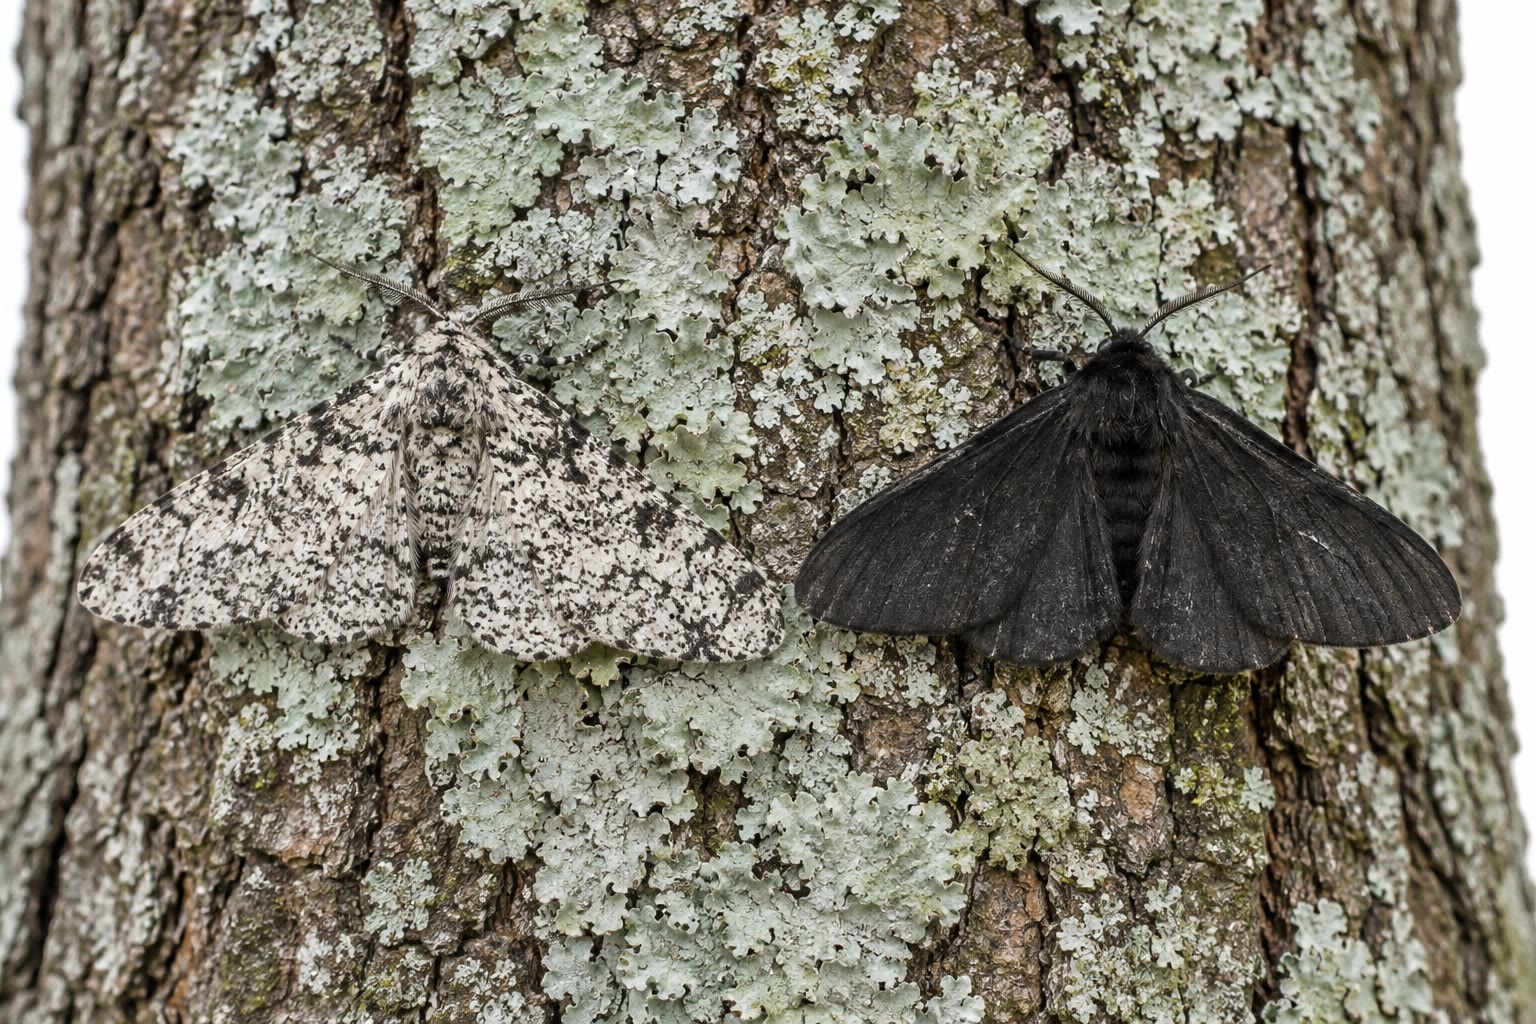
\includegraphics[width=0.46\linewidth]{images/book4/ai/b4-22-peppered-moths.jpg}\hspace{0.04\linewidth}
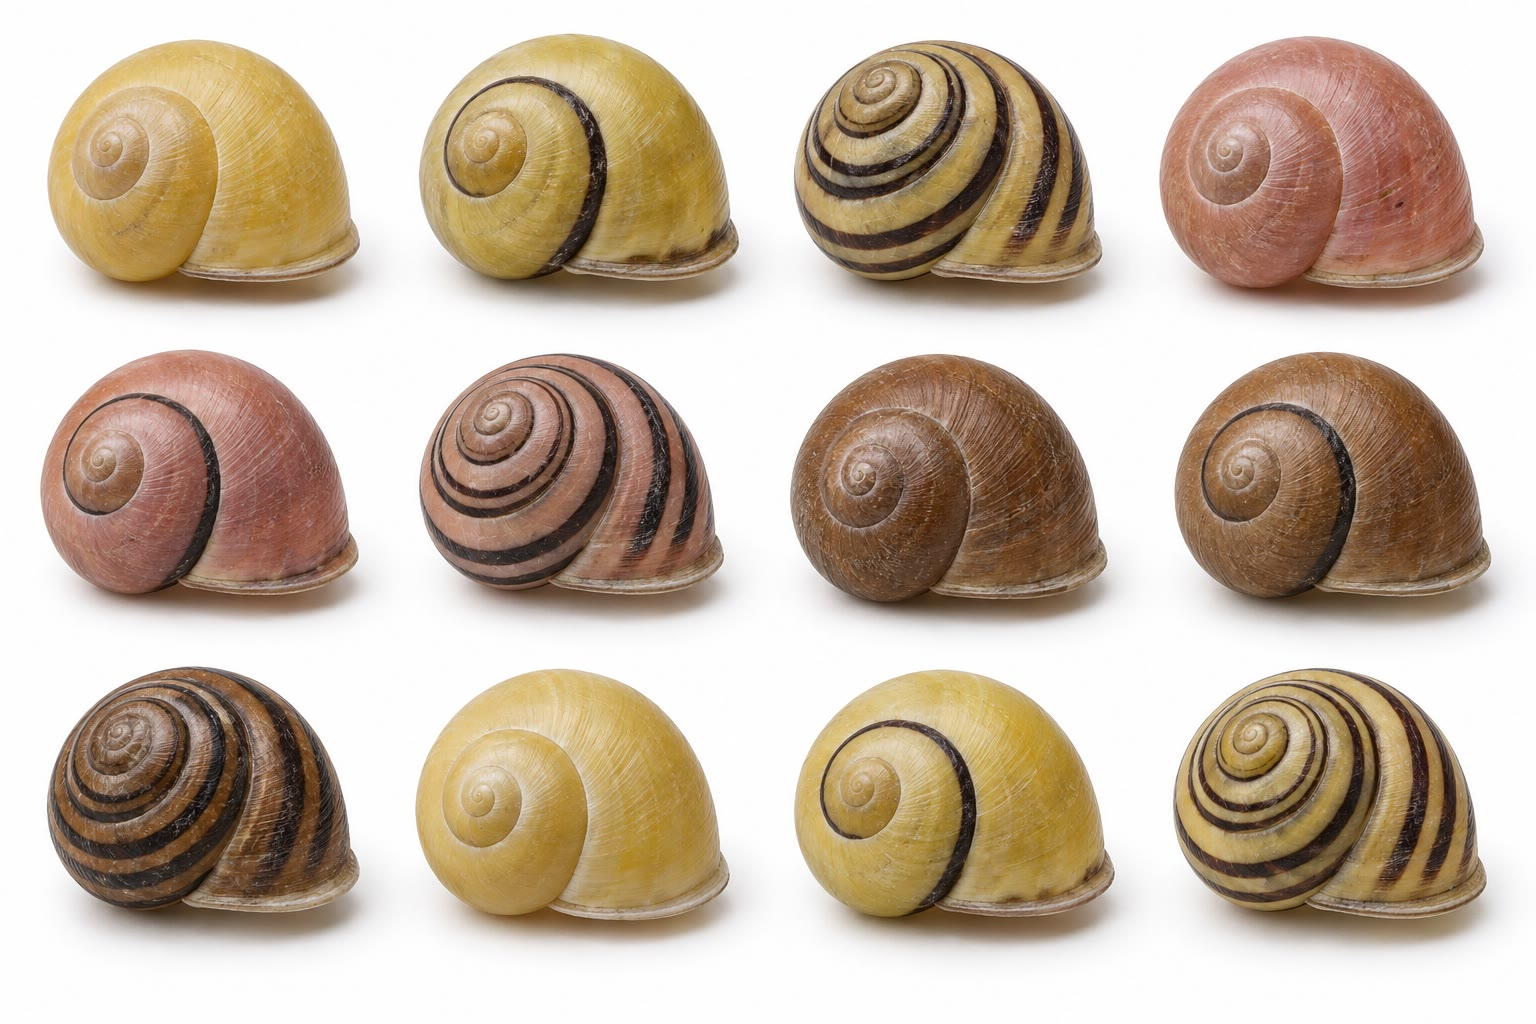
\includegraphics[width=0.46\linewidth]{images/book4/ai/b4-22-banded-snails.jpg}

{\small बाएँ: शैवाकों पर मिर्चदार पतंगे के दोनों रूप ---
कोई चिड़िया किसे पाती है यह उस \omterm{def:b2:plant-meristems:wood}{छाल} पर निर्भर है। दाएँ: कुंज-घोंघे का
कवच-बहुरूपता, जिसमें रंग तथा पट्टियाँ हर समष्टि में उन परभक्षियों से बनी
रहती हैं जो आम रूप सीख लेते हैं।}
\end{omfigure}

\section{अभ्यास}

\begin{exercise}[$\star$]\label{exo:b2:population-genetics:1}
1000 लोगों के किसी प्रतिदर्श में 640 $MM$ हैं, 320 $MN$ और 40 $NN$।
युग्मविकल्पी-बारंबारताएँ और हार्डी--वाइनबर्ग अपेक्षाएँ निकालिए।
क्या वह समष्टि साम्य में है?
\end{exercise}

\begin{exercise}[$\star$]\label{exo:b2:population-genetics:2}
वर्णकहीनता \omterm{def:b2:meiosis-heredity:vocabulary}{अप्रभावी} है और \num{20000} में से एक व्यक्ति को होती है।
\omterm{def:b2:population-genetics:frequencies}{युग्मविकल्पी बारंबारता} और वाहक-बारंबारता निकालिए।
\end{exercise}

\begin{exercise}[$\star$]\label{exo:b2:population-genetics:3}
\omterm{def:b2:population-genetics:fitness}{अनुकूलता}, \omterm{def:b2:population-genetics:fitness}{वरण गुणांक} तथा वंशागतिता की परिभाषा दीजिए, और वे
पाँच बल दीजिए जो युग्मविकल्पी-बारंबारताएँ बदलते हैं।
\end{exercise}

\begin{exercise}[$\star$]\label{exo:b2:population-genetics:4}
दिशात्मक, स्थायीकारी तथा \omterm{prop:b2:population-genetics:kinds}{संतुलनकारी वरण} का एक-एक उदाहरण दीजिए,
और हर एक में वरण का कारक।
\end{exercise}

\begin{exercise}[$\star\star$]\label{exo:b2:population-genetics:5}
किसी घातक \omterm{def:b2:meiosis-heredity:vocabulary}{अप्रभावी} \omterm{def:b2:meiosis-heredity:vocabulary}{युग्मविकल्पी} की बारंबारता $0.02$ है। उसे आधा करने में कितनी
पीढ़ियाँ? $0.001$ तक पहुँचने में? यह इस बारे में क्या कहता है कि
प्रभावित व्यष्टियों को प्रजनन से रोकने का क्या प्रभाव होगा?
\end{exercise}

\begin{exercise}[$\star\star$]\label{exo:b2:population-genetics:6}
$w_{AA} = 1$, $w_{Aa} = 1$, $w_{aa} = 0.8$ तथा $p = 0.3$ के साथ
$\bar w$, $p'$ तथा $\Delta p$ निकालिए। $p = 0.9$ के लिए दोहराइए। वह
दूसरा परिवर्तन इतना छोटा क्यों है?
\end{exercise}

\begin{exercise}[$\star\star$]\label{exo:b2:population-genetics:7}
किसी मलेरिया वाले क्षेत्र में हँसिया-कोशिका समयुग्मज की $w = 0.2$ है और सामान्य समयुग्मज
की $w = 0.88$, और विषमयुग्मजों की $w = 1$। उस हँसिया \omterm{def:b2:meiosis-heredity:vocabulary}{युग्मविकल्पी} की
साम्य बारंबारता और साम्य पर उस रोग के साथ जन्मे बच्चों का
अंश निकालिए।
\end{exercise}

\begin{exercise}[$\star\star$]\label{exo:b2:population-genetics:8}
कोई \omterm{def:b2:meiosis-heredity:vocabulary}{अप्रभावी} घातक प्रति युग्मक $\mu = \qty{2e-5}{}$ पर \omterm{def:b2:genome-diversification:mutation}{उत्परिवर्तन} से उपजता है।
उसकी साम्य बारंबारता और प्रभावित जन्मों का अंश
निकालिए। उसी दर पर कोई \omterm{def:b2:meiosis-heredity:vocabulary}{प्रभावी} घातक (प्रजनन से पहले):
जन्मों का कौन-सा अंश?
\end{exercise}

\begin{exercise}[$\star\star$]\label{exo:b2:population-genetics:9}
50 प्रजनन करते व्यष्टियों की कोई समष्टि $H = 0.5$ से शुरू होती है।
10, 50 तथा 200 पीढ़ियों बाद उसकी विषमयुग्मजता निकालिए। 100 पीढ़ियों भर
अपनी विषमयुग्मजता का \qty{90}{\%} रखने के लिए किसी समष्टि को कितना
बड़ा होना चाहिए?
\end{exercise}

\begin{exercise}[$\star\star\star$]\label{exo:b2:population-genetics:10}
किसी द्वीप का उपनिवेशन ऐसी किसी मुख्यभूमि समष्टि के 10 पक्षी करते हैं जिसमें
किसी \omterm{def:b2:meiosis-heredity:vocabulary}{युग्मविकल्पी} की बारंबारता $0.1$ है। यह प्रायिकता निकालिए कि वह
\omterm{def:b2:meiosis-heredity:vocabulary}{युग्मविकल्पी} उन संस्थापकों में नहीं है, और यह प्रायिकता कि यदि वह एक प्रति में मौजूद हो तो वह
उस द्वीप पर अंततः नियत हो जाए। मुख्यभूमि से तुलना कीजिए।
\end{exercise}

\begin{exercise}[$\star\star\star$]\label{exo:b2:population-genetics:11}
दूध-उपज की $h^{2} = 0.3$ है और मानक विचलन
\qty{1000}{L}। कोई प्रजनक ऊपर की \qty{20}{\%} गायें
माताओं के रूप में रखता है (उनका माध्य उस झुंड के माध्य से $1.4$ मानक विचलन ऊपर है)।
प्रति पीढ़ी अनुक्रिया निकालिए। यदि साँड़ ऊपर के
\qty{1}{\%} से चुने जाएँ (माध्य $2.7$ मानक विचलन ऊपर), तो वह
अनुक्रिया क्या है? बहुत पीढ़ियों बाद वह अनुक्रिया धीमी क्यों पड़ती है?
\end{exercise}

\begin{exercise}[$\star\star\star$]\label{exo:b2:population-genetics:12}
``वरण उसे नहीं देख सकता जिसे वह देख नहीं सकता।'' विषमयुग्मजों में
\omterm{def:b2:meiosis-heredity:vocabulary}{अप्रभावी} \omterm{def:b2:meiosis-heredity:vocabulary}{युग्मविकल्पी}, उदासीन \omterm{def:b2:genome-diversification:mutation}{उत्परिवर्तन}, और शून्य वंशागतिता वाले लक्षण के साथ
इस पर विचार कीजिए, कि वरण किस पर काम कर सकता है और किस पर
नहीं।
\end{exercise}

\section{समस्या: वह पतंगा, वह द्वीप और वह झुंड}

\begin{problem}[{सप्तांत समस्या --- मिर्चदार पतंगे की चढ़ाई
वरण-समीकरण से गिनी गई, किसी संस्थापक समष्टि का अपवाह
तथा अंतःप्रजनन पीछा किया गया, कोई उत्परिवर्तन--वरण संतुलन साधा गया, और किसी
प्रजनक का कार्यक्रम बताया गया, और अंत उस पतंगे के वरण गुणांक,
उस द्वीप की विषमयुग्मजता, तथा उस झुंड के लाभ पर}]
\label{pb:b2:population-genetics:1}
मिर्चदार पतंगा: काला \omterm{def:b2:meiosis-heredity:vocabulary}{युग्मविकल्पी} $M$ \omterm{def:b2:meiosis-heredity:vocabulary}{प्रभावी}, 1848 में बारंबारता $p_0 = 0.001$;
50 पीढ़ियाँ बाद पतंगों का \qty{90}{\%} काला; मानिए
$w_{MM} = w_{Mm} = 1$ और $w_{mm} = 1 - s$। द्वीप: ऐसी किसी मुख्यभूमि से 12
पक्षियों ने बसाया जहाँ $H = 0.4$ है और किसी \omterm{def:b2:meiosis-heredity:vocabulary}{अप्रभावी} हानिकर
\omterm{def:b2:meiosis-heredity:vocabulary}{युग्मविकल्पी} की $q = 0.05$; और उसके बाद वह द्वीप 40 प्रजनन करते पक्षी
थामे है। \omterm{def:b2:genome-diversification:mutation}{उत्परिवर्तन}: $\mu = \qty{1e-5}{}$। झुंड: $h^{2} = 0.4$,
मानक विचलन \qty{800}{L}।

\medskip
\noindent\textbf{भाग I --- वह पतंगा।}
\begin{enumerate}
  \item 1848 में पतंगों का कौन-सा अंश काला था, और $M$ युग्मविकल्पियों का
        कौन-सा अंश विषमयुग्मजों में बैठा था?
  \item दिखाइए कि, $M$ \omterm{def:b2:meiosis-heredity:vocabulary}{प्रभावी} होने पर, पीले \omterm{def:b2:meiosis-heredity:vocabulary}{युग्मविकल्पी} की बारंबारता
        $q' = q(1 - sq)/(1 - sq^{2})$ मानती है।
  \item $q_0 = 0.999$ से शुरू करके एक पीढ़ी बाद $q$ निकालिए, और वह भी
        $s = 0.3$ के लिए।
  \item \qty{90}{\%} काले का अर्थ है $q^{2} = 0.1$। तब $q$ क्या है?
  \item उस पुनरावर्तन से आज़माकर (या सन्निकटन
        $\Delta q \approx -sq^{2}p$ से, जब तक $q$ 1 के पास हो) पीढ़ियों की वह
        संख्या आँकिए जो $s = 0.3$ को $q$ $0.999$ से
        $0.32$ तक ले जाने में लगे, और देखी गई 50 से तुलना कीजिए।
  \item स्वच्छ-वायु क़ानूनों के बाद पीले रूप को लाभ है, और $s
        = 0.3$, जो $mm$ के विरुद्ध था, $s = 0.3$ बनकर $M\_$ के विरुद्ध हो जाता है। दिखाइए
        कि $\Delta p = -spq^{2}/\bar w$, और समझाइए कि पीले रूप की वापसी
        पहले धीमी क्यों है और $M$ के किसी चरघातांकी ह्रास में क्यों अंत होती है,
        जबकि वह चढ़ाई चरघातांकी शुरू हुई थी और
        किसी रेंगन में अंत हुई।
\end{enumerate}

\medskip
\noindent\textbf{भाग II --- वह द्वीप।}
\begin{enumerate}[resume]
  \item यह प्रायिकता निकालिए कि उन 12 संस्थापकों में से कोई भी उस
        हानिकर \omterm{def:b2:meiosis-heredity:vocabulary}{युग्मविकल्पी} को न ढोए।
  \item संस्थापन-पीढ़ी के बाद प्रत्याशित विषमयुग्मजता निकालिए
        ($H = 0.4$ से 12 व्यष्टियों ने, यानी 24
        जीन-प्रतियों ने खींची)।
  \item 100 पीढ़ियों बाद विषमयुग्मजता, मुख्यभूमि के किसी अंश के रूप में, $N =
        40$ पर निकालिए।
  \item किसी एक पक्षी में कोई उदासीन \omterm{def:b2:genome-diversification:mutation}{उत्परिवर्तन} प्रकट होता है। उसकी
        नियतन-प्रायिकता और, यदि वह नियत हो, तो नियतन तक का प्रत्याशित काल
        निकालिए।
  \item वे द्वीप-पक्षी यादृच्छिक रूप से प्रजनन करते हैं पर सब संबंधी हैं।
        $F = 1/(2N)$ के साथ, जो प्रति पीढ़ी जमा होकर 30 पीढ़ियों बाद
        लगभग $0.3$ तक पहुँचती है, $q = 0.05$ पर उस \omterm{def:b2:meiosis-heredity:vocabulary}{युग्मविकल्पी} के लिए
        प्रभावित समयुग्मजों की बारंबारता, अंतःप्रजनन के साथ तथा बिना, निकालिए।
  \item हर पीढ़ी मुख्यभूमि का एक पक्षी आता है। समझाइए कि यह
        उस द्वीप के विचलन तथा उसके भार का क्या करता है।
\end{enumerate}

\medskip
\noindent\textbf{भाग III --- वह संतुलन।}
\begin{enumerate}[resume]
  \item $\mu = 10^{-5}$ से पोसे गए किसी \omterm{def:b2:meiosis-heredity:vocabulary}{अप्रभावी} घातक की
        साम्य बारंबारता, और प्रभावित जन्मों का अंश निकालिए।
  \item $s = 0.1$ (यानी कोई हलका हानिकर \omterm{def:b2:meiosis-heredity:vocabulary}{अप्रभावी}) के लिए वही
        निकालिए।
  \item $hs = 0.05$ की \omterm{def:b2:meiosis-heredity:vocabulary}{विषमयुग्मजी} हानि वाले किसी \omterm{def:b2:meiosis-heredity:vocabulary}{प्रभावी} \omterm{def:b2:meiosis-heredity:vocabulary}{युग्मविकल्पी}
        के लिए साम्य निकालिए।
  \item चिकित्सा उस घातक को ठीक कर देती है ताकि $s$ गिरकर $0.1$ हो जाए।
        वह साम्य कैसे बदलता है, और वहाँ पहुँचने में उस समष्टि को कितना
        (परिमाण की कोटि में) समय लगता है?
  \item उस जीनोम में \num{20000} जीन हैं जिनमें से हर एक $10^{-5}$ पर
        किसी \omterm{def:b2:meiosis-heredity:vocabulary}{अप्रभावी} घातक में उत्परिवर्तित होता है। कोई औसत व्यक्ति \omterm{def:b2:meiosis-heredity:vocabulary}{विषमयुग्मजी} दशा में
        कितने \omterm{prop:b2:meiosis-heredity:extensions}{घातक युग्मविकल्पी} ढोता है? (साम्य पर
        हर स्थल पर प्रति व्यक्ति $2\hat q$ प्रतियाँ हैं।)
  \item समझाइए कि वह संख्या किसी स्वस्थ समष्टि के अनुकूल क्यों है और
        वह चचेरों के विवाह को महँगा क्यों बना देती है।
\end{enumerate}

\medskip
\noindent\textbf{भाग IV --- वह झुंड।}
\begin{enumerate}[resume]
  \item वह प्रजनक ऊपर की \qty{30}{\%} गायें रखता है (माध्य उस झुंड से $1.16$
        मानक विचलन ऊपर)। लीटरों में वरण
        अंतर और वह अनुक्रिया निकालिए।
  \item उसी वरण की पाँच पीढ़ियों बाद प्रत्याशित लाभ क्या है, और
        असली लाभ छोटा क्यों हो सकता है?
  \item साँड़ आधे जीन देते हैं और ऊपर के
        \qty{2}{\%} ($2.4$ मानक विचलन) से वरे जाते हैं। जब गायें तथा साँड़ ऊपर की तरह
        वरे जाएँ तब वह अनुक्रिया निकालिए (दोनों अंतरों का औसत लीजिए)।
  \item ऐसा कोई झुंड जहाँ सारी गायें किसी एक प्राणी के \omterm{def:b2:asexual-reproduction:clone}{क्लोन} हों: उसमें
        $h^{2}$ और वह अनुक्रिया क्या हैं? यह वंशागतिता के बारे में
        क्या कहता है?
  \item किसी फ़िंच समष्टि की चोंच-गहराई के लिए $h^{2} = 0.7$ है और
        वह सूखा ऐसे बचे हुए छोड़ता है जो \qty{0.6}{mm} गहरे हैं। अगली पीढ़ी बताइए।
  \item वह प्रजनक $h^{2} = 0.1$ वाले किसी लक्षण की ओर मुड़ता है। मानक
        विचलनों में कौन-सा वरण अंतर प्रश्न 19 जितनी ही अनुक्रिया देता है?
  \item परिणाम बताइए: उस पतंगे की $s$ और \qty{90}{\%} काले तक का काल,
        100 पीढ़ियों बाद उस द्वीप की विषमयुग्मजता,
        और उस झुंड की प्रति पीढ़ी अनुक्रिया।
\end{enumerate}
\end{problem}
